\documentclass[times,specification,annotation]{itmo-student-thesis}

%% Опции пакета:
%% - specification - если есть, генерируется задание, иначе не генерируется
%% - annotation - если есть, генерируется аннотация, иначе не генерируется
%% - times - делает все шрифтом Times New Roman, собирается с помощью xelatex
%% - languages={...} - устанавливает перечень используемых языков. По умолчанию это {english,russian}.
%%                     Последний из языков определяет текст основного документа.

%% Делает запятую в формулах более интеллектуальной, например:
%% $1,5x$ будет читаться как полтора икса, а не один запятая пять иксов.
%% Однако если написать $1, 5x$, то все будет как прежде.
\usepackage{icomma}

%% Один из пакетов, позволяющий делать таблицы на всю ширину текста.
\usepackage{tabularx}

%% Данные пакеты необязательны к использованию в бакалаврских/магистерских
%% Они нужны для иллюстративных целей
%% Начало
\usepackage{tikz}
\usetikzlibrary{arrows}
\usepackage{filecontents}
\begin{filecontents}{bachelor-thesis.bib}
@online{late-fusion-cnn,
    year        = {2019},
    title       = {A Late Fusion CNN for Digital Matting},
    author      = {Yunke Zhang, Lixue Gong},
    url         = {https://openaccess.thecvf.com/content_CVPR_2019/papers/Zhang_A_Late_Fusion_CNN_for_Digital_Matting_CVPR_2019_paper.pdf},
    langid      = {english}
}

@online{pose2seg,
    year        = {2019},
    title       = {Pose2Seg: Detection Free Human Instance Segmentation},
    author      = {Song-Hai Zhang, Ruilong Li},
    url         = {https://arxiv.org/abs/1803.10683},
    langid      = {english}
}

@online{fba,
    year        = {2020},
    title       = {F, B, Alpha Matting},
    author      = {Marco Forte, François Pitié},
    url         = {https://arxiv.org/abs/2003.07711},
    langid      = {english}
}

@online{trimap-free-matting,
    year        = {2020},
    title       = {Is a Green Screen Really Necessary for Real-Time Human Matting?},
    author      = {Zhanghan Ke, Kaican Li},
    url         = {https://arxiv.org/abs/2011.11961v1},
    langid      = {english}
}

@online{deepfashion2,
    year        = {2019},
    title       = {DeepFashion2: A Versatile Benchmark for Detection, Pose Estimation, Segmentation and Re-Identification of Clothing Images},
    author      = {Yuying Ge, Ruimao Zhang},
    url         = {https://arxiv.org/abs/1901.07973},
    langid      = {english}
}

@online{dsfd,
    year        = {2019},
    title       = {DSFD: Dual Shot Face Detector},
    author      = {Jian Li, Yabiao Wang},
    url         = {https://arxiv.org/abs/1810.10220},
    langid      = {english}
}

@online{mask-rcnn,
    year        = {2018},
    title       = {Mask R-CNN},
    author      = {Kaiming He, Georgia Gkioxari},
    url         = {https://arxiv.org/abs/1703.06870},
    langid      = {english}
}
\end{filecontents}
%% Конец

%% Указываем файл с библиографией.
\addbibresource{bachelor-thesis.bib}

\begin{document}

\studygroup{M3437}
\title{Детализированная сегментация изображения человека и генерация нового изображения}
\author{Пенская Таисия Андреевна}{Пенская Т.А.}
\supervisor{Фильченков Андрей Александрович}{Фильченков А.А.}{к.ф.-м.наук}{доцент ФИТиП, Университет ИТМО}
\publishyear{2021}
%% Дата выдачи задания. Можно не указывать, тогда надо будет заполнить от руки.
\startdate{15}{февраля}{2020}
%% Срок сдачи студентом работы. Можно не указывать, тогда надо будет заполнить от руки.
\finishdate{31}{мая}{2021}
%% Дата защиты. Можно не указывать, тогда надо будет заполнить от руки.
% \defencedate{ }{ }{2021}

\addconsultant{Ефимова В.А.}{без степени, без звания}

\secretary{Павлова О.Н.}

%% Задание
%%% Техническое задание и исходные данные к работе
\technicalspec{Требуется сгенерировать новое изображение человека на основе детализированной сегментации существующего изображения человека, соответствующее данному текстовому описанию. Изначально сервису подается на вход которому подается JSON определенного вида на английском языке, по которому сервис должен возвращать RGBA изображение человека, соответствующее описанию.}

%%% Содержание выпускной квалификационной работы (перечень подлежащих разработке вопросов)
\plannedcontents{\begin{enumerate}
    \item Найти сегментацию лица и одежды с помощью существующих моделей.
    \item Вырезать человека из остального изображения с помощью alpha mating.
    \item Реализовать генерацию произвольного человека с помощью StyleGAN2.
    \item Сгенерировать новую сегментацию по отличительным признакам.
    \item По сегментации сгенерировать изображение человека.
    \item Сравнить результаты с результатами существующих методов по метрикам FID, IS, SOA.
\end{enumerate}}

%%% Исходные материалы и пособия 
\plannedsources{\begin{enumerate}
    \item Маттинг изображений: https://arxiv.org/pdf/2011.11961v1.pdf.
    \item Pix2Pix: https://arxiv.org/pdf/1611.07004.pdf.
    \item Pix2PixHD: https://arxiv.org/pdf/1711.11585.pdf
    \item CPGAN: https://arxiv.org/pdf/1912.08562.pdf.
    \item Метрика для оценки качества: https://arxiv.org/pdf/1910.13321.pdf.
\end{enumerate}}

%%% Цель исследования
\researchaim{Разработка и реализация алгоритма генерации изображения человека на основе детализированной сегментации существующего изображения человека, соответствующее данному текстовому описанию.}

%%% Задачи, решаемые в ВКР
\researchtargets{\begin{enumerate}
    \item Разработка алгоритма для детализированной сегментации изображения человека.
    \item Разработка алгоритма генерации новой позы человека по текстовому описанию.
    \item Разработка алгоритма генерации изображения по текстовому описанию и сегментации, основанной на новой позе человека.
    \item Генерация набора данных для оценки качества работы алгоритма.
\end{enumerate}}

%%% Использование современных пакетов компьютерных программ и технологий
\addadvancedsoftware{\texttt{latex}}{\ref{sec:1}}
\addadvancedsoftware{\texttt{python3} скрипты}{}

%%% Краткая характеристика полученных результатов 
\researchsummary{Разработан и реализован алгоритм для детализированной сегментации изображения человека. Сгенерирован датасет высокого качества с единственным человеком на изображении.}

%%% Гранты, полученные при выполнении работы 
\researchfunding{Нет}

%%% Наличие публикаций и выступлений на конференциях по теме выпускной работы
\researchpublications{Нет}

%% Эта команда генерирует титульный лист и аннотацию.
\maketitle{Бакалавр}

%% Оглавление
\tableofcontents

%% Макрос для введения. Совместим со старым стилевиком.
\startprefacepage

Компьютерное зрение — это научное направление в области искусственного интеллекта и связанные с ним технологии получения изображений объектов реального мира, их обработки и использования полученных данных для решения разного рода прикладных задач без участия (полного или частичного) человека.

Одной из популярных задач компьютерного зрения является задача автоматического создания изображений на основе текста. Качественное решение этой задачи может быть использовано в любой литературе, ведь читателю проще воспринимать текст, который сопровождается иллюстрацией.

В последнее время (2017-2020) появилось много видов порождающих состязательных сетей (англ. Generative Adversarial Networks, GANs), решающих ее. Однако несмотря на рост популярности этой задачи, текущие модели генерируют нереалистичные изображения низкого качества. 
Данную задачу можно разбить на несколько подзадач, в числе которых будет генерация нового изображения человека по существующему. Это позволит создавать изображения несуществующих людей, не защищенные авторским правом.

Целью настоящей работы является разработка и реализация алгоритма генерации изображения человека на основе детализированной сегментации существующего изображения человека, соответствующее данному текстовому описанию.

Предлагаемый алгоритм принимает на вход фотографию и текстовое описание, в виде JSON, на английском языке. После этого, первым важным этапом нашей задачи является извлечение человека из фотографии. Чтобы качественно отделить человека от остального изображения, было принято использовать alpha matting. Следующим этапом обработки изображений является его детализированная сегментация, а именно сегментация лица и одежды человека. Дальнейшим шагом является генерация новой сегментации по отличительным признакам, указанным в описании. Конечным этапом является генерация нового изображения по полученной сегментации. 

Данный подход позволит получать изображения людей в высоком разрешении, соответствующие данному текстовому описанию. Результаты можно будет использовать во многих сферах: игровая индустрия, киноиндустрия, научные исследования и многое другое. 

%% Начало содержательной части.
\chapter{Обзор современных результатов и постановка задачи}

\section{Алгоритмы для сегментации изображений}\label{sec:1}

Фундаментальной задачей компьютерного зрения является задача поиска групп пикселей, каждая из которых характеризует один смысловой объект, на изображениях и видео. 
Различают два типа подхода для данной задачи: сегментация и матирование.

Сегментация изображения — это задача кластеризации частей изображения на группы, посредством предсказания на уровне пикселей. То есть, сегментация изображения генерирует двоичное изображение, в котором пиксель либо принадлежит одной группе, либо другой.

Матирование изображения отличается от сегментации изображения тем, что некоторые пиксели могут принадлежать как одной группе, так и другой, такие пиксели называются частичными или смешанными пикселями. Чтобы полностью отделить передний план от фона в изображении, необходима точная оценка альфа-значений для частичных или смешанных пикселей.

В данной работе эта задача будет использована для выделения человека на изображении и детализированного выделения его одежды и лица.

\subsection{Алгоритмы для сегментации человека полностью}

Важной частью данной работы является выделение человека на изображении, чтобы впоследствии вырезать его и упростить задачу для генеративно-состязательных сетей, подавая на вход изображение без фона. 
Для сегментации и маттинга человека существует множество решений, которые были проанализированы,  подробнее о них в следующей таблице~\ref{tab1}.

\begin{table}[!h]
\caption{Таблица существующих решений для выделения человека на изображении.}\label{tab1}
\centering
\begin{tabular}{|l|l|}
\hline
Статья              & Комментарии                                                                                                                                                                       \\ \hline
\cite{late-fusion-cnn}     & Используется tensorflow.                                                                                                                                                          \\ \hline
\cite{pose2seg}            & \begin{tabular}[c]{@{}l@{}}Делается сегментация, что грубее, чем маттинг, \\ а значит, конечные результаты будут хуже. \\ Отдельно для своих данных нужно выделять keypoints.\end{tabular} \\ \hline
\cite{fba}                 & Нужна дополнительно сгенерированная тримапа.                                                                                                                                      \\ \hline
\cite{trimap-free-matting} & \begin{tabular}[c]{@{}l@{}}Недавно полученные хорошие результаты, \\ предобученная модель есть.\end{tabular}                                                                      \\ \hline
\end{tabular}
\end{table}

\subsection{Алгоритмы для детализированной сегментации человека}

Для сегментации одежды на человеке был найден хороший датасет DeepFashion2\cite{deepfashion2}, который и был использован для обучении модели впоследствии.

Для сегментации лица человека была найдена предобученная модель\cite{dsfd} с хорошими результатами, которая была использована дальше в реализации алгоритма.

\section{Алгоритмы для трансляции изображения}\label{sec:2}

Важной задачей компьтерного зрения является также задача трансляции изображения, цель которой состоит в том, чтобы научиться строить соответствия между входным и выходным изображениями, используя тренировочные данные. 

Для решения этой задачи используются такие архитектуры, как генеративно-состязательные сети.
Генеративно-состязательные сети — алгоритм машинного обучения, входящий в семейство порождающих моделей и построенный на комбинации из двух нейронных сетей: генеративная модель $G$, которая строит приближение распределения данных, и дискриминативная модель $D$, оценивающая вероятность, что образец пришел из тренировочных данных, а не сгенерированных моделью $G$. Обучение для модели $G$ заключается в максимизации вероятности ошибки дискриминатора $D$.

В данной работе этот подход используется для генерации нового изображения человека по сегментации и отличительным признакам, указанным в тексте.

\section{Постановка задачи}\label{sec:2}

В качестве достижения поставленной цели диплома были поставлены следующие подзадачи:
\begin{enumerate}
    \item Разработка алгоритма для детализированной сегментации изображения человека.
    \item Разработка алгоритма генерации новой позы человека.
    \item Разработка алгоритма генерации изображения по текстовому описанию и сегментации, основанной на новой позе человека.
    \item Генерация набора данных для оценки качества работы алгоритма
\end{enumerate}

\chapter{Описание разработанных алгоритмов}

\section{Подробное описание предполагаемого решения}

Для решения поставленной задачи был придуман следующий алгоритм:
\begin{enumerate}
    \item Вырезать человека из изображения с помощью alpha mating.
    \item Сегментировать лицо и одежду.
    \item Реализовать генерацию новой позы человека по тексту (человек сидит/стоит).
    \item Сгенерировать новую сегментацию по позе человека.
    \item По сегментации сгенерировать изображение человека по отличительным признакам, релевантным тестовому описанию.
\end{enumerate}

\section{Алгоритм для детализированной сегментации изображения человека}

Для осуществления детализированной сегментации нужно поэтапно сделать следующее:
\begin{enumerate}
    \item{Вырезать человека полностью из изображения с помощью матирования}
    \item{Сегментировать лицо и одежду}
\end{enumerate}

Для сегментации человека была выбрана модель с лучшими показателями\cite{trimap-free-matting} из таблицы\ref{tab1}.

Для сегментации лица человека была использована предобученная модель\cite{dsfd}.

Для сегментации одежды человека была обучена Mask-RCNN\cite{mask-rcnn} с использованием датасета DeepFashion2\cite{deepfashion2}.

\section{Алгоритм генерации новой сегментации по текстовому описанию}

Для генерации новой сегментации по текстовому описанию:
\begin{enumerate}
    \item{Определить текущую позу человека}
    \item{По тексту определить новую позу человеку}
    \item{Сгенерировать сегментацию для новой позы человека}
\end{enumerate}

\chapter{Полученные результаты алгоритмов}

В результате была обучена Mask-RCNN, результаты ниже на графике:

\begin{figure}[h]
\center{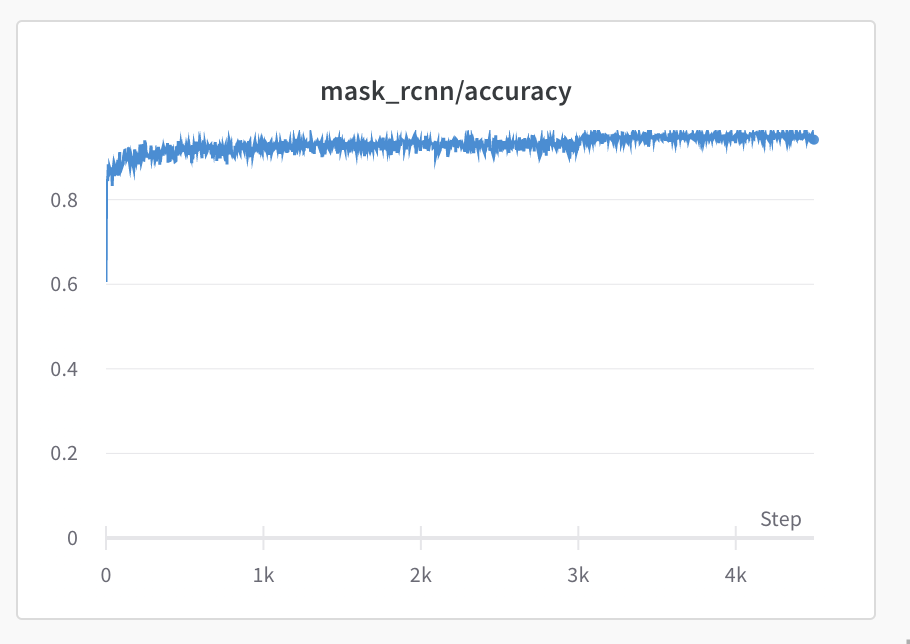
\includegraphics[scale=0.8]{images/mask-rcnn.png}}
\caption{Mask-RCNN результаты}
\label{fig:image}
\end{figure}

Был предобработан датасет Fashionpedia, в результате чего был получен датасет с 31188 качественными изображениями с человеком, а 17695 изображений были удалены.

%% Макрос для заключения. Совместим со старым стилевиком.
\startconclusionpage

В процессе.

\printmainbibliography

%% После этой команды chapter будет генерировать приложения, нумерованные русскими буквами.
%% \startappendices из старого стилевика будет делать то же самое
\appendix

\end{document}
